% \documentclass{standalone}
% \usepackage[usenames,dvipsnames,table,tikz]{xcolor} % use colors on table and more
% \usepackage{tikz}
%
% \usepackage{pgfplots}
% \begin{document}
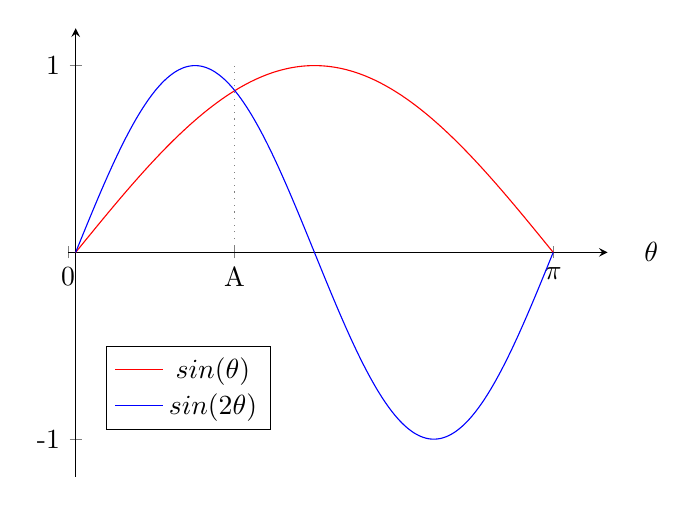
\begin{tikzpicture}\begin{axis}[axis lines=middle,samples=200
        ,xlabel=$\theta$
        ,ymax=1.2
        ,ymin=-1.2
        ,xmin = -0.05
        ,xmax = 3.5
        ,every axis x label/.style={
          at={(ticklabel* cs:1.05)},
            anchor=west,
          },
        every axis y label/.style={
          at={(ticklabel* cs:1.05)},
            anchor=south,
          },
        ,xtick=data
        ,xtick={-0.05,1.045,3.141592}
        ,xticklabels={0,A,$\pi$}
        ,ytick=data,
        ,ytick={1,-1}
        ,yticklabels={1,-1}
        ,legend style={at={(axis cs:0.2,-0.5)},anchor=north west}
        ]
      \addplot[red,domain=0:3.141592] {sin(deg(x)};
      \addplot[blue,domain=0:3.141592] {sin(deg(2*x))};
      \addplot[gray,dotted,mark=none] coordinates {(1.045, 0) (1.045, 1)};
      \legend{$sin(\theta$),$sin(2\theta$)}
\end{axis}\end{tikzpicture}
% \end{document}
